\chapter{Resultados}
\label{chap:resultados}

Os resultados obtidos com o desenvolvimento desse projeto são apresentados e discutidos nesse capítulo de forma divida em três seções.  
A primeira e a segunda sobre os modelos do DT1 e da pista do Kartódromo de Sonoma. E a última  sobre os resultados da solução do OCP proposto.

\section{Modelo do veículo DT1}
\label{sec:resultados_modelo}

O modelo obtido para o veículo para o veículo DT1 foi a Equação (\ref{eq:modelo_1}) e o conjunto de constates da Tabela \ref{tab:constantes}.
Entretanto esse modelo não foi validado experimentalmente pois esse projeto foi realizado, em sua maior parte, durante o regime de ensino remoto
emergência causado pela pandemia de Covid-19 em 2020. Na solução do OCP proposto a marca de consumo calculado para a estratégia ótima
foi de $905,7$ [km/kWh] que é um valor muito distante das marcas realmente realizas pelo DT1 de $266,5$ [km/kWh] em 2018 e de $226,9$ [km/kWh] em 2019  no Kartódromo de Sonoma na Shell Eco-marathon Americas. 
Apesar de que uma melhora na marca era esperada, esta grande diferença entre os valores das marcas deve ser analisada com ceticismo, ela indica que as constantes do modelo podem precisar ser ajustadas e/ou as simplificações revistas.


\section{Modelo da pista}
\label{sec:resultados_pista}

A curva ajustada para representar a altitude relativa em função da distância  apresentou um erro maior nos pontos que a distância  percorrida esta entre 290 e 575 e metros e entre 1005 e 1265 metros. O máximo erro destes
intervalos foi de 19\% e 34\% respetivamente. Ja no restante do intervalo o erro máximo ficou abaixo de 10\%. 
O modelo de inclinação, obtido a partir do arco  tangente da derivada desta curva, foi aprestando na Equação (\ref{eq:modeloTheta}). 
A Figura \ref{graf:modelo_pista} apresenta uma comparação entre os dados de altitude e a curva ajusta.
e o comportamento periódico desejado na curva ajustada para descrever a repetição das voltas na tentativa.

\begin{figure}[h]
    \centering
    \caption{Curva ajustada para representar altitude da pista}
    \input{Resultados/Figuras/pista.tex}
    \label{graf:modelo_pista}
    \caption*{\footnotesize{Fonte: Elaborada pelo autor.}}
\end{figure}


% \begin{figure}[H]
%     \centering
%     \caption{Curva ajustada para representar altitude da pista}
%     \input{Resultados/Figuras/pista_modelo.tex}
%     \label{graf:modelo_pista}
%     \caption*{\footnotesize{Fonte: Elaborada pelo autor.}}
% \end{figure}

% \begin{figure}[H]
%     \centering
%     \caption{Representação da periodicidade da curva ajusta}
%     % This file was created by matlab2tikz.
%
%The latest updates can be retrieved from
%  http://www.mathworks.com/matlabcentral/fileexchange/22022-matlab2tikz-matlab2tikz
%where you can also make suggestions and rate matlab2tikz.
%
\definecolor{mycolor1}{rgb}{0.00000,0.44700,0.74100}%
%
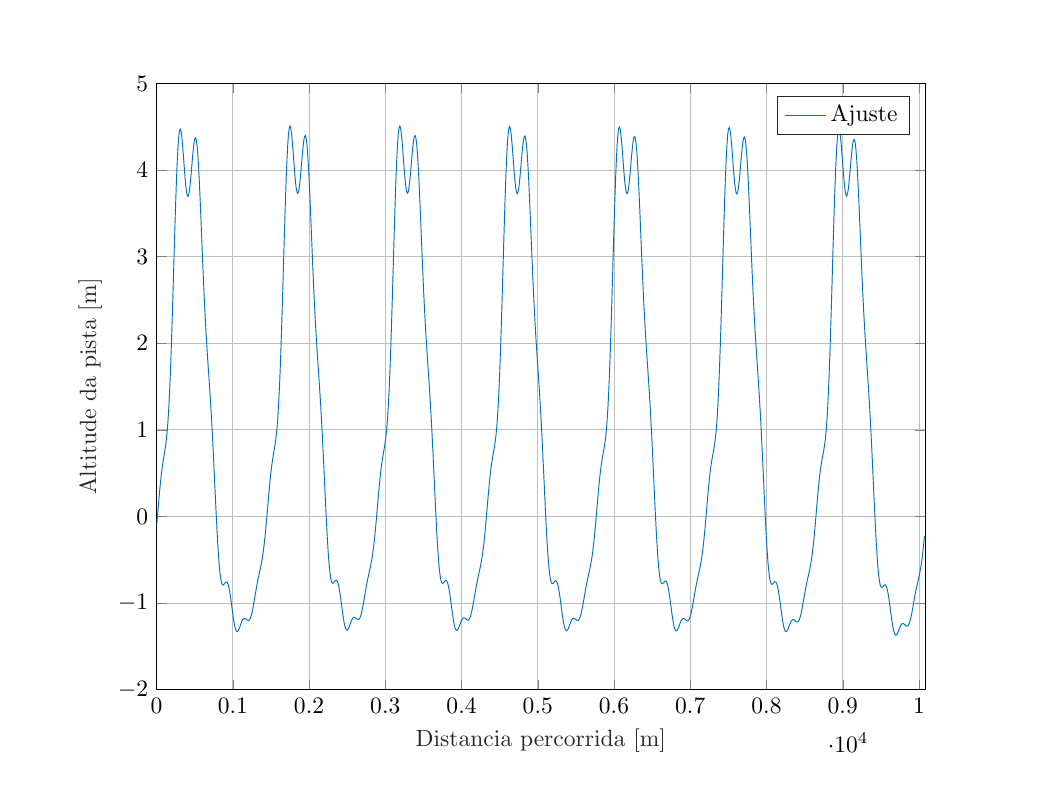
\begin{tikzpicture}[scale=0.85]

\begin{axis}[%
width=4.521in,
height=3.566in,
at={(0.758in,0.481in)},
scale only axis,
xmin=0,
xmax=10080,
xlabel style={font=\color{white!15!black}},
xlabel={Distancia percorrida [m]},
ymin=-2,
ymax=5,
ylabel style={font=\color{white!15!black}},
ylabel={Altitude da pista [m]},
axis background/.style={fill=white},
xmajorgrids,
ymajorgrids,
legend style={legend cell align=left, align=left, draw=white!15!black}
]
\addplot [color=mycolor1]
  table[row sep=crcr]{%
1	-0.109711917352081\\
11	-0.00839975833814072\\
21	0.0950935994183011\\
31	0.197575097473076\\
41	0.295906341954157\\
51	0.387379176406482\\
61	0.470078639152616\\
71	0.543194918667103\\
81	0.607248810660309\\
91	0.664201673014787\\
101	0.717430477656014\\
111	0.771560468559376\\
121	0.832161105813\\
131	0.90532420971175\\
141	0.997155276962692\\
151	1.11321865673269\\
161	1.25798366412261\\
171	1.43432106813152\\
181	1.64309736617324\\
191	1.88290788488262\\
201	2.14997946131707\\
211	2.43826005992245\\
221	2.73969727047449\\
231	3.04469152045332\\
241	3.34269442603896\\
251	3.62290937310388\\
261	3.87504138340178\\
271	4.09003753619072\\
281	4.26075828112619\\
291	4.38252407940657\\
301	4.45349069459108\\
311	4.47481944853005\\
321	4.45062481979224\\
331	4.38769956903536\\
341	4.29503563665075\\
351	4.18317584164875\\
361	4.06344547969927\\
371	3.94712305498246\\
381	3.84461469530785\\
391	3.76469681065797\\
401	3.71388623172202\\
411	3.69598683386881\\
421	3.71184736196174\\
431	3.75934802063559\\
441	3.83361482784037\\
451	3.92744231294103\\
461	4.03188842668885\\
471	4.13699192257323\\
481	4.23255310092945\\
491	4.30891444440015\\
501	4.35767864845305\\
511	4.37230773581937\\
521	4.34855776398591\\
531	4.28471812059516\\
541	4.18164127523908\\
551	4.04256664568099\\
561	3.8727594054464\\
571	3.6790001416205\\
581	3.46897299806302\\
591	3.25060734872116\\
601	3.03143056535272\\
611	2.81798693557988\\
621	2.61537055476623\\
631	2.42690877308266\\
641	2.25401858405504\\
651	2.09624249436254\\
661	1.95145434447245\\
671	1.81621068151138\\
681	1.68621091627265\\
691	1.55682067929601\\
701	1.42360824671759\\
711	1.28284396176586\\
721	1.13191714177985\\
731	0.969633539600276\\
741	0.796368175204486\\
751	0.614062149913995\\
761	0.426066616015826\\
771	0.236851065707892\\
781	0.051605264766321\\
791	-0.124226585294145\\
801	-0.28543530967372\\
811	-0.427514275401029\\
821	-0.547062158447048\\
831	-0.642084803994541\\
841	-0.712169858877593\\
851	-0.758519932931108\\
861	-0.783843217554211\\
871	-0.792113527366725\\
881	-0.788223438901982\\
891	-0.777563525199437\\
901	-0.765566810209672\\
911	-0.757259984130101\\
921	-0.756861473257333\\
931	-0.767461349089345\\
941	-0.790809830657308\\
951	-0.827230601643877\\
961	-0.875663350222557\\
971	-0.933827967298308\\
981	-0.998491826252851\\
991	-1.06581252391888\\
1001	-1.13172219610016\\
1011	-1.19231656474594\\
1021	-1.24421244050807\\
1031	-1.28484137061795\\
1041	-1.31265404530945\\
1051	-1.32721924116057\\
1061	-1.32921157058291\\
1071	-1.32029309615128\\
1081	-1.30290391790131\\
1091	-1.27998520033189\\
1101	-1.25466400050152\\
1111	-1.22993216571023\\
1121	-1.20835126193031\\
1131	-1.19181206044295\\
1141	-1.18137094078277\\
1151	-1.17717731518708\\
1161	-1.17849669058402\\
1171	-1.18382421671065\\
1181	-1.19107449731941\\
1191	-1.19782596034705\\
1201	-1.20159292065635\\
1211	-1.20009611694053\\
1221	-1.19150317027772\\
1231	-1.17461400061693\\
1241	-1.14897236222076\\
1251	-1.11489268027755\\
1261	-1.07340046056913\\
1271	-1.02609376840127\\
1281	-0.974941685251106\\
1291	-0.922042386510245\\
1301	-0.869367844030426\\
1311	-0.818523683801552\\
1321	-0.770551248021045\\
1331	-0.725794552227129\\
1341	-0.683848015544151\\
1351	-0.643592252309563\\
1361	-0.603315711498686\\
1371	-0.560910505351947\\
1381	-0.514122357766729\\
1391	-0.460828114779785\\
1401	-0.399310403671038\\
1411	-0.328498261776184\\
1421	-0.248145037368798\\
1431	-0.158920426954973\\
1441	-0.0624016779830519\\
1451	0.0390409958153942\\
1461	0.142458819696212\\
1471	0.244621962609591\\
1481	0.342373910009698\\
1491	0.433009194713195\\
1501	0.514636725900871\\
1511	0.586490261571256\\
1521	0.649150627850389\\
1531	0.70465094198183\\
1541	0.756445837883422\\
1551	0.809237707503833\\
1561	0.868666201312164\\
1571	0.940880473947201\\
1581	1.03202567577401\\
1591	1.14768481484112\\
1601	1.29232337115105\\
1611	1.46878624345062\\
1621	1.67789440831694\\
1631	1.91818212523839\\
1641	2.1858050795613\\
1651	2.4746363321751\\
1661	2.7765514538704\\
1671	3.0818880808922\\
1681	3.38004974341147\\
1691	3.66021056250047\\
1701	3.91206749718755\\
1711	4.12658119495929\\
1721	4.29664574188969\\
1731	4.41763189133126\\
1741	4.48775740399173\\
1751	4.50825126801585\\
1761	4.48329473066804\\
1771	4.41973993115163\\
1781	4.32662498083452\\
1791	4.21452106172837\\
1801	4.09476107417914\\
1811	3.97860935253988\\
1821	3.87643710676308\\
1831	3.79696807207257\\
1841	3.74665334488901\\
1851	3.72922399418815\\
1861	3.7454556265135\\
1871	3.7931618592856\\
1881	3.86741507237606\\
1891	3.96097443033605\\
1901	4.06488454615074\\
1911	4.16919468741892\\
1921	4.26373922867053\\
1931	4.33891587951821\\
1941	4.38639938307744\\
1951	4.3997347376935\\
1961	4.3747649568976\\
1971	4.30986296522801\\
1981	4.20595414475607\\
1991	4.06633382285708\\
2001	3.89630109056\\
2011	3.70264530253945\\
2021	3.49303317666715\\
2031	3.27535163586291\\
2041	3.05706386130738\\
2051	2.84463333293164\\
2061	2.64306324088849\\
2071	2.45558728891871\\
2081	2.28353364450786\\
2091	2.12636792910063\\
2101	1.98190511329033\\
2111	1.84666540848799\\
2121	1.7163370160708\\
2131	1.58629994863694\\
2141	1.45216078056107\\
2151	1.31024842651069\\
2161	1.15802577978455\\
2171	0.994380758508237\\
2181	0.819772148019413\\
2191	0.63621946571085\\
2201	0.447140621642194\\
2211	0.257055072709677\\
2221	0.0711822165349781\\
2231	-0.105026119306842\\
2241	-0.266374844844081\\
2251	-0.408390936247001\\
2261	-0.52772236817059\\
2271	-0.622434877067988\\
2281	-0.692180725667297\\
2291	-0.738225775326999\\
2301	-0.763334352315229\\
2311	-0.771524388431763\\
2321	-0.767716935020035\\
2331	-0.757313347586203\\
2341	-0.745739411463418\\
2351	-0.737997933651879\\
2361	-0.7382697204275\\
2371	-0.749597612541098\\
2381	-0.773679911866189\\
2391	-0.810788934937414\\
2401	-0.859818595970919\\
2411	-0.918452978348607\\
2421	-0.9834369141028\\
2431	-1.05092065765553\\
2441	-1.11684460981355\\
2451	-1.17732724078422\\
2461	-1.22902007508595\\
2471	-1.26939769943262\\
2481	-1.29695778207113\\
2491	-1.31131532379874\\
2501	-1.31318587487361\\
2511	-1.30426321938879\\
2521	-1.28700701334462\\
2531	-1.26436412045858\\
2541	-1.23945315760302\\
2551	-1.21524452852757\\
2561	-1.19426777701328\\
2571	-1.17837453046989\\
2581	-1.1685790351634\\
2591	-1.16498996650145\\
2601	-1.16683768558383\\
2611	-1.17259136664965\\
2621	-1.18015141108624\\
2631	-1.18709518087878\\
2641	-1.19094904643271\\
2651	-1.18945752987899\\
2661	-1.18082112945581\\
2671	-1.163878124775\\
2681	-1.13821188746484\\
2691	-1.10417330744339\\
2701	-1.06281705745925\\
2711	-1.01575962122082\\
2721	-0.964975358495653\\
2731	-0.912553514665536\\
2741	-0.860443314589362\\
2751	-0.810215664323673\\
2761	-0.762868359004461\\
2771	-0.71869720512976\\
2781	-0.677248546929054\\
2791	-0.637360026867475\\
2801	-0.597286881858604\\
2811	-0.554901651476558\\
2821	-0.507946828414134\\
2831	-0.454313597483903\\
2841	-0.392316088042783\\
2851	-0.32092995139631\\
2861	-0.239966711702738\\
2871	-0.150161045476146\\
2881	-0.0531564291649808\\
2891	0.0486153042655554\\
2901	0.152154000824888\\
2911	0.254193570256236\\
2921	0.351560026288614\\
2931	0.441551312851706\\
2941	0.522300934601968\\
2951	0.593086875477846\\
2961	0.654550515125696\\
2971	0.708797066931038\\
2981	0.759358941488504\\
2991	0.811015556340023\\
3001	0.869476400370953\\
3011	0.940947410493913\\
3021	1.03161268752164\\
3031	1.14707310812312\\
3041	1.29178951328604\\
3051	1.46858018988898\\
3061	1.67821998581917\\
3071	1.91918167958509\\
3081	2.18754962831664\\
3091	2.47712207229177\\
3101	2.77970290432061\\
3111	3.08556754338769\\
3121	3.38407219379886\\
3131	3.66436259362606\\
3141	3.91612856605821\\
3151	4.13034521696469\\
3161	4.29994104254356\\
3171	4.42033767516037\\
3181	4.48981521803792\\
3191	4.50967039565048\\
3201	4.48415100883931\\
3211	4.42016809033865\\
3221	4.32680520673144\\
3231	4.21466101621697\\
3241	4.09507504098498\\
3251	3.97929645047824\\
3261	3.87766061455082\\
3271	3.79883782313765\\
3281	3.74921288521327\\
3291	3.73244377411941\\
3301	3.74923295617508\\
3311	3.79732774518316\\
3321	3.87174742517548\\
3331	3.96521654733918\\
3341	4.06876728002307\\
3351	4.17246036019907\\
3361	4.26616516957475\\
3371	4.34033547371321\\
3381	4.38671871661783\\
3391	4.39894329435757\\
3401	4.37293933330678\\
3411	4.3071631763426\\
3421	4.20261273892485\\
3431	4.06263865658181\\
3441	3.89257317190016\\
3451	3.69921354891173\\
3461	3.49020820883375\\
3471	3.27340082063725\\
3481	3.05618971294326\\
3491	2.84495709652224\\
3501	2.64461503596073\\
3511	2.45830362736606\\
3521	2.28726250410126\\
3531	2.1308809180206\\
3541	1.98691565929691\\
3551	1.8518514011584\\
3561	1.72136596576967\\
3571	1.59085453256746\\
3581	1.45596263994659\\
3591	1.31307825849592\\
3601	1.15973811531745\\
3611	0.994912300750151\\
3621	0.819143120439789\\
3631	0.634528032965973\\
3641	0.444551044677242\\
3651	0.253780789344372\\
3661	0.067465453952224\\
3671	-0.108936328528585\\
3681	-0.270244277566914\\
3691	-0.412019541837268\\
3701	-0.530959746561425\\
3711	-0.625190629127377\\
3721	-0.694428927063916\\
3731	-0.740003375712762\\
3741	-0.764733857930665\\
3751	-0.772681697365916\\
3761	-0.768795614412628\\
3771	-0.758486934206376\\
3781	-0.747173456839254\\
3791	-0.739833492203418\\
3801	-0.740609799003622\\
3811	-0.752497782021677\\
3821	-0.777143858212993\\
3831	-0.814769239760178\\
3841	-0.864222532183184\\
3851	-0.923152632602985\\
3861	-0.988282548629893\\
3871	-1.05575593642078\\
3881	-1.12152216306434\\
3891	-1.18172304029534\\
3901	-1.2330452376257\\
3911	-1.27300661210768\\
3921	-1.30015182191712\\
3931	-1.31414188744043\\
3941	-1.31573289867114\\
3951	-1.30664981102404\\
3961	-1.2893711898497\\
3971	-1.26684891960167\\
3981	-1.24219253384207\\
3991	-1.21835044847344\\
4001	-1.1978197932734\\
4011	-1.18241285119381\\
4021	-1.17310174602351\\
4031	-1.16995463817434\\
4041	-1.17216715502379\\
4051	-1.17818305848217\\
4061	-1.18588920790449\\
4071	-1.19286259337564\\
4081	-1.19664230167593\\
4091	-1.19499720194536\\
4101	-1.1861610808664\\
4111	-1.16901079597025\\
4121	-1.14316933894755\\
4131	-1.10902384946087\\
4141	-1.0676577531166\\
4151	-1.02070537634236\\
4161	-0.970145672985785\\
4171	-0.918058229257204\\
4181	-0.866368817033628\\
4191	-0.816613005865686\\
4201	-0.769744574766057\\
4211	-0.726010844066624\\
4221	-0.684910024423064\\
4231	-0.645236952226242\\
4241	-0.605214027510975\\
4251	-0.562694766890764\\
4261	-0.515419104674251\\
4271	-0.461293297230767\\
4281	-0.398663699763548\\
4291	-0.326553224018508\\
4301	-0.244832078074922\\
4311	-0.154300239894579\\
4321	-0.0566675192038929\\
4331	0.0455727546647442\\
4341	0.149369386827174\\
4351	0.251420549341063\\
4361	0.348535438860226\\
4371	0.43801613507362\\
4381	0.518021462428984\\
4391	0.587874283886948\\
4401	0.648277049708184\\
4411	0.701407398116836\\
4421	0.750875621708201\\
4431	0.801538031519352\\
4441	0.859173593767532\\
4451	0.930044467953282\\
4461	1.02037299678602\\
4471	1.13577713279455\\
4481	1.28071227468474\\
4491	1.45796935967078\\
4501	1.66827650581806\\
4511	1.91004460591045\\
4521	2.17928652306115\\
4531	2.46972577130372\\
4541	2.77309491764668\\
4551	3.07960774777241\\
4561	3.37857390822608\\
4571	3.65911164116987\\
4581	3.9109045630591\\
4591	4.12494312733209\\
4601	4.29419101003624\\
4611	4.41412130287145\\
4621	4.48307678853789\\
4631	4.50242198846714\\
4641	4.47647103250519\\
4651	4.41219335336525\\
4661	4.31871725034078\\
4671	4.20666796676953\\
4681	4.0873906626068\\
4691	3.97211834925178\\
4701	3.87114963927479\\
4711	3.79310061457673\\
4721	3.74428925339168\\
4731	3.72830015534106\\
4741	3.74576265609394\\
4751	3.79435806025612\\
4761	3.86905310750416\\
4771	3.96253849399793\\
4781	4.06583484054178\\
4791	4.16901530948211\\
4801	4.26198522019608\\
4811	4.33525521774953\\
4821	4.38064609247041\\
4831	4.39187005086318\\
4841	4.36494447888093\\
4851	4.29840900944683\\
4861	4.1933337038751\\
4871	4.05312389808791\\
4881	3.88314421678459\\
4891	3.69019897482842\\
4901	3.48191742914298\\
4911	3.26609919799272\\
4921	3.05007710428843\\
4931	2.84015163896252\\
4941	2.64114353254819\\
4951	2.45609932428189\\
4961	2.28617041640072\\
4971	2.13067021610322\\
4981	1.98729802936202\\
4991	1.85250379249395\\
5001	1.72195577913788\\
5011	1.59106511764574\\
5021	1.45551697068141\\
5031	1.31175884148751\\
5041	1.15740153965532\\
5051	0.99149732503302\\
5061	0.814671769383148\\
5071	0.629099789858731\\
5081	0.438330822075135\\
5091	0.246981886079804\\
5101	0.0603291160437442\\
5111	-0.116162866917553\\
5121	-0.277329310060742\\
5131	-0.418766089329753\\
5141	-0.537220822197283\\
5151	-0.630879345724785\\
5161	-0.699522720430722\\
5171	-0.744542168499829\\
5181	-0.768812543414552\\
5191	-0.77643783019091\\
5201	-0.772393610273662\\
5211	-0.76210036636017\\
5221	-0.750967170276958\\
5231	-0.743947226880766\\
5241	-0.745144827455544\\
5251	-0.757507744184746\\
5261	-0.782630549922456\\
5271	-0.820683622954029\\
5281	-0.870470731289588\\
5291	-0.929606210591703\\
5301	-0.99479196170474\\
5311	-1.06216578441959\\
5321	-1.12768670827949\\
5331	-1.18752047223153\\
5341	-1.23838931245838\\
5351	-1.27785457667711\\
5361	-1.30450791418447\\
5371	-1.31805615030916\\
5381	-1.31929550819321\\
5391	-1.30998155813075\\
5401	-1.29261112467127\\
5411	-1.27014043391958\\
5421	-1.24566929528688\\
5431	-1.22212359738301\\
5441	-1.20196767103155\\
5451	-1.18697426226862\\
5461	-1.17807339173284\\
5471	-1.17529293472056\\
5481	-1.17779420370248\\
5491	-1.18399611608134\\
5501	-1.19177265158176\\
5511	-1.19870112164413\\
5521	-1.20233398658379\\
5531	-1.20046501983181\\
5541	-1.19136169939746\\
5551	-1.17393966917773\\
5561	-1.14786153323961\\
5571	-1.11355045593862\\
5581	-1.07211819273916\\
5591	-1.02521633013662\\
5601	-0.974827727368291\\
5611	-0.923021580649208\\
5621	-0.871699504103512\\
5631	-0.822361118090603\\
5641	-0.775915722528825\\
5651	-0.732561882075727\\
5661	-0.691749623454086\\
5671	-0.65223115090478\\
5681	-0.612196409817006\\
5691	-0.569480448737413\\
5701	-0.521821319121635\\
5711	-0.467141081524286\\
5721	-0.403819037629839\\
5731	-0.330926000139338\\
5741	-0.248391360738889\\
5751	-0.157080710186729\\
5761	-0.0587702847557871\\
5771	0.0439852237341798\\
5781	0.148083927953945\\
5791	0.250188792131437\\
5801	0.347092856381779\\
5811	0.436103063773211\\
5821	0.515404282722282\\
5831	0.584364905130815\\
5841	0.643748963145229\\
5851	0.695806840655715\\
5861	0.744226808470209\\
5871	0.793941929590395\\
5881	0.850800277683937\\
5891	0.921119667893307\\
5901	1.011159971315\\
5911	1.12655542147619\\
5921	1.271755172588\\
5931	1.44952207862169\\
5941	1.66053693379028\\
5951	1.90314834984942\\
5961	2.17329754111752\\
5971	2.46463340145052\\
5981	2.76881753564511\\
5991	3.07600269022259\\
6001	3.37545273019981\\
6011	3.656259294355\\
6021	3.9081007238689\\
6031	4.12198370809991\\
6041	4.29090786883547\\
6051	4.41039833106196\\
6061	4.47886088571468\\
6071	4.49772790263973\\
6081	4.471379606938\\
6091	4.40684332952534\\
6101	4.31329137350302\\
6111	4.20137467243125\\
6121	4.08244303908869\\
6131	3.96771233603063\\
6141	3.8674435067867\\
6151	3.79019767061393\\
6161	3.74222544191348\\
6171	3.72703777993521\\
6181	3.74519091099121\\
6191	3.79430043593274\\
6201	3.86928111097238\\
6211	3.96279054259811\\
6221	4.06583870523537\\
6231	4.16851214344749\\
6241	4.26075304238937\\
6251	4.3331297448767\\
6261	4.37753702534393\\
6271	4.38777130422695\\
6281	4.35993736394961\\
6291	4.29265798971039\\
6301	4.1870749929942\\
6311	4.04664779638075\\
6321	3.87677263408077\\
6331	3.68426001332165\\
6341	3.47671916247087\\
6351	3.26190485882661\\
6361	3.04708377558004\\
6371	2.83847424421572\\
6381	2.6408054648315\\
6391	2.45703048271724\\
6401	2.28821278321631\\
6411	2.13359046321988\\
6421	1.99080604758482\\
6431	1.85627554080943\\
6441	1.72565849925616\\
6451	1.59438277965339\\
6461	1.45817382375786\\
6471	1.31353913658475\\
6481	1.15816384991459\\
6491	0.991182380977039\\
6501	0.813303304567194\\
6511	0.626778506348153\\
6521	0.4352221789461\\
6531	0.243298935633004\\
6541	0.0563120162181395\\
6551	-0.120268783558876\\
6561	-0.281294950527896\\
6571	-0.42239763380241\\
6581	-0.540374774359932\\
6591	-0.633472396556515\\
6601	-0.70153572122028\\
6611	-0.746018060524634\\
6621	-0.769848644848614\\
6631	-0.77717338488352\\
6641	-0.77299391283215\\
6651	-0.762739057602265\\
6661	-0.751808423263048\\
6671	-0.745129507602381\\
6681	-0.746767722214123\\
6691	-0.759623018490201\\
6701	-0.785238174383896\\
6711	-0.823733012168367\\
6721	-0.87386693919754\\
6731	-0.93322035773951\\
6741	-0.998474779967866\\
6751	-1.06576288867175\\
6761	-1.13105406663915\\
6771	-1.19053855787688\\
6781	-1.24097457724413\\
6791	-1.27996717273519\\
6801	-1.30615497509042\\
6811	-1.31929038980985\\
6821	-1.32020935804754\\
6831	-1.31069750224054\\
6841	-1.29326925241673\\
6851	-1.27088449661721\\
6861	-1.24663268151009\\
6871	-1.22341663376531\\
6881	-1.20366750708417\\
6891	-1.18911832614556\\
6901	-1.18065703615198\\
6911	-1.17827146502713\\
6921	-1.18108903564423\\
6931	-1.18750439313141\\
6941	-1.19537930179836\\
6951	-1.20229208664139\\
6961	-1.20580923474658\\
6971	-1.20374997459447\\
6981	-1.19441586979588\\
6991	-1.17676154907852\\
7001	-1.15048921068425\\
7011	-1.1160578084506\\
7021	-1.07460699575215\\
7031	-1.02780502950524\\
7041	-0.977637981160131\\
7051	-0.926163924454248\\
7061	-0.875259612208226\\
7071	-0.826388106781589\\
7081	-0.780413772084764\\
7091	-0.737486155146442\\
7101	-0.697007056617631\\
7111	-0.657686230503229\\
7121	-0.617681556658883\\
7131	-0.574810175445773\\
7141	-0.526808933487088\\
7151	-0.471616427767162\\
7161	-0.407645623721687\\
7171	-0.334015869348012\\
7181	-0.250716231079849\\
7191	-0.158678213566937\\
7201	-0.0597445617627375\\
7211	0.0434688150042029\\
7221	0.147809695550517\\
7231	0.249906374477391\\
7241	0.346536401770879\\
7251	0.435012314442613\\
7261	0.513545748882924\\
7271	0.58155127266305\\
7281	0.639855005254393\\
7291	0.690780389188819\\
7301	0.738093760638044\\
7311	0.786804783693372\\
7321	0.842830260918894\\
7331	0.912543089050261\\
7341	1.00223994928583\\
7351	1.11757055938818\\
7361	1.26297702811862\\
7371	1.44119339704165\\
7381	1.65285254976734\\
7391	1.89624043131084\\
7401	2.16722646355438\\
7411	2.45938503801703\\
7421	2.76430717231811\\
7431	3.07208517813766\\
7441	3.37193792328874\\
7451	3.6529313410688\\
7461	3.90473943112655\\
7471	4.11838600618794\\
7481	4.28690739578024\\
7491	4.40588132572593\\
7501	4.47377691574696\\
7511	4.49209442642569\\
7521	4.46527993526424\\
7531	4.400418161491\\
7541	4.30672467685665\\
7551	4.19487520652659\\
7561	4.07622323047485\\
7571	3.9619664741243\\
7581	3.86232730580276\\
7591	3.78581113579335\\
7601	3.73860069188631\\
7611	3.72413303781792\\
7621	3.74289132358689\\
7631	3.79242576274579\\
7641	3.86759969829595\\
7651	3.96103841935221\\
7661	4.06374215910588\\
7671	4.16581180191836\\
7681	4.25722732434861\\
7691	4.3286155798219\\
7701	4.37194595695006\\
7711	4.38109948435756\\
7721	4.35226846800225\\
7731	4.2841586981622\\
7741	4.17798333274786\\
7751	4.03725526139993\\
7761	3.86740155221951\\
7771	3.67523804653447\\
7781	3.46835308341198\\
7791	3.25445581554871\\
7801	3.04074613164843\\
7811	2.83335977527225\\
7821	2.63693423183279\\
7831	2.45432912774566\\
7841	2.28652035687543\\
7851	2.13267124948148\\
7861	1.99036825914209\\
7871	1.85599426732478\\
7881	1.72520094479848\\
7891	1.59343365339373\\
7901	1.45645876325882\\
7911	1.31084424261564\\
7921	1.15434977611166\\
7931	0.986191916808387\\
7941	0.807161970594909\\
7951	0.619588294202077\\
7961	0.427149159872773\\
7971	0.234555978707817\\
7981	0.0471382553501445\\
7991	-0.129629849521732\\
8001	-0.290616767448686\\
8011	-0.431489457692471\\
8021	-0.549096505539075\\
8031	-0.64174419916296\\
8041	-0.709341746213374\\
8051	-0.753404142381356\\
8061	-0.776914393574985\\
8071	-0.78405959540548\\
8081	-0.779866618407227\\
8091	-0.769771827220102\\
8101	-0.759164622340435\\
8111	-0.752946198467872\\
8121	-0.755142682906191\\
8131	-0.768606026551919\\
8141	-0.794827270057781\\
8151	-0.833875964981332\\
8161	-0.884467640493358\\
8171	-0.944149396724428\\
8181	-1.00958307563319\\
8191	-1.07689697975942\\
8201	-1.14207153047971\\
8211	-1.20132204683009\\
8221	-1.25144312467191\\
8231	-1.29008371120361\\
8241	-1.3159293981306\\
8251	-1.32877793633509\\
8261	-1.32950456143636\\
8271	-1.31992437914831\\
8281	-1.30256876786739\\
8291	-1.2804005974098\\
8301	-1.25649831553355\\
8311	-1.23374115727839\\
8321	-1.21452672796891\\
8331	-1.20054815460003\\
8341	-1.19265134310186\\
8351	-1.19078431965754\\
8361	-1.19404104934135\\
8371	-1.20079248162257\\
8381	-1.20888883138123\\
8391	-1.21591012826711\\
8401	-1.21943753540864\\
8411	-1.21731628054999\\
8421	-1.20788239857789\\
8431	-1.19012969157679\\
8441	-1.16379992332827\\
8451	-1.12938759190208\\
8461	-1.08805980784403\\
8471	-1.04150090203569\\
8481	-0.991699460684102\\
8491	-0.940701701124891\\
8501	-0.890358812759513\\
8511	-0.842096695216966\\
8521	-0.796734325721692\\
8531	-0.754371979419795\\
8541	-0.714363197083409\\
8551	-0.675375472459833\\
8561	-0.635535015902263\\
8571	-0.59264162446658\\
8581	-0.544431620444267\\
8591	-0.488860869090527\\
8601	-0.42437671347977\\
8611	-0.350147665068909\\
8621	-0.266222947654343\\
8631	-0.173600270670087\\
8641	-0.0741889588387081\\
8651	0.029334016950841\\
8661	0.133766470226962\\
8671	0.235702572313187\\
8681	0.331905055122274\\
8691	0.419692782874768\\
8701	0.497304883520215\\
8711	0.564202743597134\\
8721	0.62127506928774\\
8731	0.670918666695638\\
8741	0.716978015286696\\
8751	0.764539219899451\\
8761	0.819587424681491\\
8771	0.888550026756298\\
8781	0.977759794334847\\
8791	1.09288113073782\\
8801	1.23834829957129\\
8811	1.41686580522804\\
8821	1.62901804120995\\
8831	1.87302790960728\\
8841	2.14469290726212\\
8851	2.43751305283213\\
8861	2.74300916305842\\
8871	3.05121372906064\\
8881	3.35130141361612\\
8891	3.63231334755117\\
8901	3.88392012472716\\
8911	4.0971635675009\\
8921	4.26511747098089\\
8931	4.38341272272904\\
8941	4.45058208338723\\
8951	4.46819373728526\\
8961	4.44075936223278\\
8971	4.37542054766766\\
8981	4.28143539250787\\
8991	4.16950351116048\\
9001	4.05098106444816\\
9011	3.9370466548522\\
9021	3.8378831748886\\
9031	3.76193958774887\\
9041	3.71533022204889\\
9051	3.70141800223998\\
9061	3.72061304662164\\
9071	3.77040050869587\\
9081	3.84559289760919\\
9091	3.93878396405898\\
9101	4.04096510882081\\
9111	4.1422525140611\\
9121	4.23266487057928\\
9131	4.30288834959105\\
9141	4.34496757598024\\
9151	4.35286857134679\\
9161	4.32287128222323\\
9171	4.25376434719113\\
9181	4.14683185865955\\
9191	4.00563954778157\\
9201	3.8356445378355\\
9211	3.64366714612535\\
9221	3.43727396512377\\
9231	3.22412774583121\\
9241	3.0113609668279\\
9251	2.80502636626579\\
9261	2.60966954257118\\
9271	2.42805679028131\\
9281	2.26107674811657\\
9291	2.10781853241108\\
9301	1.96581324173337\\
9311	1.83141144666797\\
9321	1.70025776416936\\
9331	1.56781583483287\\
9341	1.42989360066487\\
9351	1.28311994656556\\
9361	1.12532933146248\\
9371	0.955820413072912\\
9381	0.775466947419435\\
9391	0.586673257344062\\
9401	0.393181012063504\\
9411	0.199747622672146\\
9421	0.0117280184922139\\
9431	-0.165400080810512\\
9441	-0.326522750100184\\
9451	-0.467343286995707\\
9461	-0.584761231633036\\
9471	-0.677143201659642\\
9481	-0.744462207517106\\
9491	-0.78829451263121\\
9501	-0.811676289767742\\
9511	-0.818835073994697\\
9521	-0.814822159982188\\
9531	-0.805080638858982\\
9541	-0.794988975757328\\
9551	-0.7894214726074\\
9561	-0.792364575784742\\
9571	-0.806622064732274\\
9581	-0.833633309021319\\
9591	-0.873417882386367\\
9601	-0.924647924063045\\
9611	-0.984837866629531\\
9621	-1.05063060077145\\
9631	-1.11815078304702\\
9641	-1.18339055345956\\
9651	-1.2425908683301\\
9661	-1.2925830973638\\
9671	-1.33106027543809\\
9681	-1.35675492421612\\
9691	-1.36950989546535\\
9701	-1.37023928765588\\
9711	-1.36078711515073\\
9721	-1.34370104459822\\
9731	-1.32194624736828\\
9741	-1.29858953894479\\
9751	-1.27648603836314\\
9761	-1.25799943856238\\
9771	-1.24478280093972\\
9781	-1.23764003702797\\
9791	-1.23647962501759\\
9801	-1.24036251066657\\
9811	-1.24763652895464\\
9821	-1.25614101324343\\
9831	-1.26345838798365\\
9841	-1.26718513781449\\
9851	-1.26519302759362\\
9861	-1.25585294076593\\
9871	-1.23819803160341\\
9881	-1.21200959064062\\
9891	-1.17781740521239\\
9901	-1.13681559386255\\
9911	-1.09070395855907\\
9921	-1.04147289893599\\
9931	-0.991156040975843\\
9941	-0.941578310392307\\
9951	-0.894127843829391\\
9961	-0.849577787757336\\
9971	-0.80797889922967\\
9981	-0.768636433971275\\
9991	-0.730175823784505\\
10001	-0.690692012705508\\
10011	-0.647968024570274\\
10021	-0.599740340505644\\
10031	-0.543982825652031\\
10041	-0.479177911405949\\
10051	-0.40454389486101\\
10061	-0.32019063148132\\
10071	-0.227182316423454\\
};
\addlegendentry{Ajuste}

%\addlegendentry{Termino da volta}

\end{axis}

\begin{axis}[%
width=5.833in,
height=4.375in,
at={(0in,0in)},
scale only axis,
xmin=0,
xmax=1,
ymin=0,
ymax=1,
axis line style={draw=none},
ticks=none,
axis x line*=bottom,
axis y line*=left
]
\end{axis}
\end{tikzpicture}%
%     \label{graf:pista_voltas}
%     \caption*{\footnotesize{Fonte: Elaborada pelo autor.}}
% \end{figure}

\section{estratégia de pista ótima}
\label{sec:resultados_otimo}
 
O código desenvolvido, conforme descrito na Seção \ref{sec:OCPporposto}, para solução o problema de controle ótimo proposto na Equação 
(\ref{eq:ObjOCP_final}) gerou um problema de programação não linear com 3005 variáveis de otimização.
Foram gastos para a execução de todo o programa $\sim 14.4$ segundos onde $\sim 7,2$ segundos deste foram utilizados na otimização do NLP em $636$ iterações da biblioteca IPOP e reposta não violou nenhuma das restrições. 
A sequência de controle ótima de $i$ e os estados gerados por ela $x$ e $v$ estão apresentados nos gráficos da Figura \ref{graf:resultadoOCP}. 
Os parâmetros otimizados tempo final $T$ e raio do eixo do motor $r_m$ são exibidos na Tabela \ref{tab:resultadoOCP} junto das métricas marca, velocidade media e velocidade final. 

\begin{table}[h]
	\centering
	\caption{Parâmetros otimizados e métricas da estratégia ótima}
	\rowcolors{1}{}{lightgray}
	\begin{tabular}{lll}
		\toprule
		\textbf{Constante} & \textbf{Unidade} & \textbf{Valor}\\
		\hline
		Marca                               & [$km/kWh$]   & 905.68  \\
        Raio do eixo do motor               & [$mm$]       & 27.56   \\
        Tempo total de prova                & [$s$]        & 1400.0  \\  
        Velocidade média                    & [$km/h$]     & 25.92   \\
        Velocidade final                    & [$km/h$ ]    & 17.09   \\
		\bottomrule
	\end{tabular}
	\caption*{\footnotesize Fonte: Elaborada pelo autor.}
	\label{tab:resultadoOCP}
\end{table}

\begin{figure}[H]
    \centering
    \caption{sequência de controle ótima $i$ e estados $v$ e $x$ correspondentes}
    \input{Resultados/Figuras/resultadoOPC.tex}
    \label{graf:resultadoOCP}
    \caption*{\footnotesize{Fonte: Elaborada pelo autor.}}
\end{figure}

A estratégia de pista ótima encontrada se assemelha muito a estratégia estratégia \textit{start-stop}, na qual o motor é desligado quando a velocidade é máxima
km/h e religado apenas quando é minima. Entretanto, no caso ótimo estes valores diferem na primeira, na última e nas demais voltas. Para a primeira volta a máxima e a mínima são
$26,8$ e $17,3$ [km/h]. Na última  os valores máximo e a mínimo são $33,2$ e $11,9$ [km/h]. Enquanto nas demais voltas os valores máximo e mínimo são $35,0$ e $17,3$ [km/h]

Nos gráficos da Figura \ref{graf:resultadotensao} estão retratos a tensão que deve ser aplicada no motor para produzir a corrente elétrica da sequência de controle ótima e a inclinação da pista em cada instante de tempo.
A partir desta pode-se observar que o motor é ligado somente no maior pico positivo de inclinação, ou seja, o motor só é ligado na maior subida pista.

Como apresentado nos gráficos da Figura \ref{graf:resultadoForcas} a maior força resistiva que atuou no veículo foi a componente do peso paralela a pista $F_g$, variando entre $-18,45$ [N] a $25,84$ [N]. Apesar de $F_g$ ser conservativa
e realizar um trabalho nulo em um circuito fechado, ela influencia fortemente, dado sua magnitude comparada as outras forças resistivas, as acelerações do protótipo e consequentemente a região de trabalho do motor.
Já o arrasto aerodinâmico $F_a$ atingiu um máximo de $2,46$ [N] e a resistência ao rolamento $F_r$ teve o valor constante de $2,02$ [N].  

\begin{figure}[h]
    \centering
    \caption{Tensão necessária para a sequência de controle ótima e inclinação da pista}
    \input{Resultados/Figuras/resultado_tensao.tex}
    \label{graf:resultadotensao}
    \caption*{\footnotesize{Fonte: Elaborada pelo autor.}}
\end{figure}

\begin{figure}[h]
    \centering
    \caption{Força tração das forças resistivas na estratégia de pista ótima}
    \input{Resultados/Figuras/resultado_forcas.tex}
    \label{graf:resultadoForcas}
    \caption*{\footnotesize{Fonte: Elaborada pelo autor.}}
\end{figure}







\clearpage